\section{Vision as LoRA}
\label{sec:methods}
\begin{figure*}
    \centering
    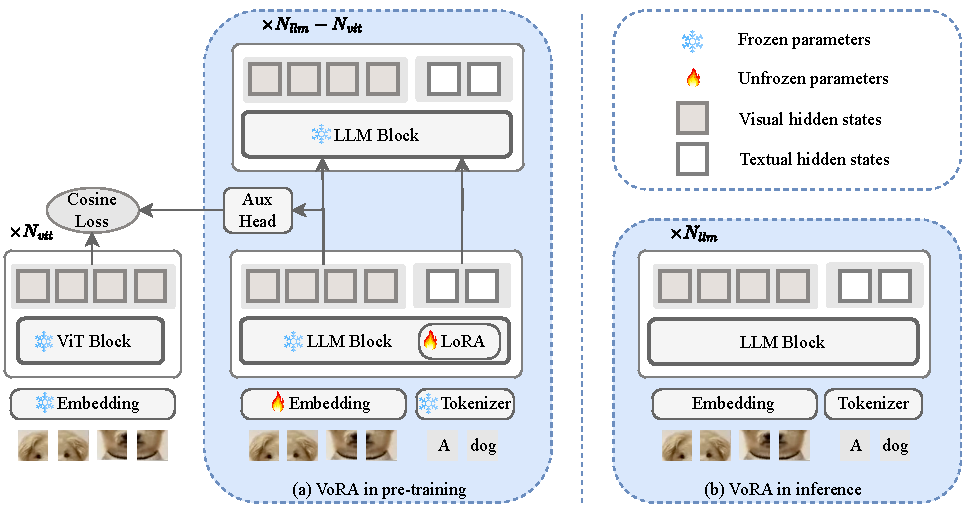
\includegraphics[width=\linewidth]{images/Figure2.pdf}
    \caption{The architecture of \model{}. Figure (a) shows the architecture of \model{} in pre-training: in this stage, \model{} only unfreezes the LoRA layers for vision and the visual embedding layer, i.e., a shallow MLP layer with a positional embedding. Figure (b) shows \model{} in inference: the LoRA layers are merged into the LLM, and thus the only added parameters are a shallow embedding layer (about 6M parameters).}
    \label{fig:architecture}
\end{figure*}
In this section, we introduce three key components of \model{}: vision as LoRA, block-wise distillation, and bi-directional attention masks for vision. 

\subsection{Stabilize training: Vision as LoRA}

As shown in Figure \ref{fig:architecture}(a), we integrate LoRA layers into the LLM to enable vision understanding. During pre-training, images are first converted into vision embeddings using a lightweight embedding layer, i.e., a shallow MLP with positional encodings of about 6M parameters. Let $N_{\text{vit}}$ and $N_{\text{llm}}$ denote the number of blocks in the ViT and the LLM, respectively. We apply LoRA to all linear layers within the first $N_{\text{vit}}$ blocks of the LLM, including query-key-value (QKV) projections and feed-forward network (FFN) layers. Crucially, only the LoRA parameters and the vision embedding layer are updated during training, while the original LLM parameters remain frozen. This design decouples vision and language parameters, stabilizing training compared to full LLM training and avoiding the training collapse observed in prior works \cite{eve}.

Figure \ref{fig:architecture}(b) demonstrates that after pre-training, the LoRA parameters can be seamlessly merged into the base LLM, thereby eliminating additional inference overhead. 

% \subsection{Boost training: Block-wise distillation}
% \label{sec:distillation}

% Our framework introduces a block-wise distillation paradigm that aligns \model{}'s emerging visual representations with the hierarchical feature spaces of a pre-trained Vision Transformer (ViT). This strategic alignment harnesses the ViT's rich visual priors to accelerate training while mitigating dependence on large-scale multimodal datasets.  


% Our core idea is to align \model{}’s visual representations with those of a pre-trained ViT, leveraging the ViT’s strong visual priors to boost training and reduce reliance on large-scale training data. To achieve this, we adopt knowledge distillation \cite{distillation}, transferring visual knowledge from the ViT into \model{}. Unlike traditional distillation methods that train an entire model, our approach updates only the LoRA layers for vision within the LLM. This ensures that the LoRA layers directly learn visual knowledge from the ViT while maintaining the LLM’s original capabilities. Specifically, for block $i$ among the first $N_{vit}$ blocks in LLM, we align its output hidden states with those of block $i$ in the ViT.
% Additionally, we require \model{} to predict a caption given an image, providing additional supervision. 
% The training objective consists of the following three components.

% \textbf{Distillation Loss.} For each transformer block $i$ and visual embedding position $s$, we compute cosine similarity between projected LLM features and ViT embeddings:
% \begin{equation}
%     \mathcal{L}_{\text{distill}}^i = \frac{1}{S} \sum_{s=1}^S \left( 1 - \frac{
%         \mathrm{AuxHead}(\bm{h}_{\text{LLM}}^{i,s})^\top \bm{h}_{\text{ViT}}^{i,s}
%     }{
%         \|\mathrm{AuxHead}(\bm{h}_{\text{LLM}}^{i,s})\|_2 \|\bm{h}_{\text{ViT}}^{i,s}\|_2
%     } \right),
% \end{equation}
% where $S$ is visual sequence length, i.e. the vision token count of the ViT, $\bm{h}_{\text{LLM}}^{i,s}, \bm{h}_{\text{ViT}}^{i,s} \in \mathbb{R}^M$ are visual hidden states for the $s$-th token in block $i$, and $\mathrm{AuxHead}(\cdot)$ is a shallow head consisting of an RMSNorm layer and a linear layer. The distillation loss is averaged across $N_{\text{ViT}}$ blocks:
% \begin{equation}
%     \mathcal{L}_{\text{distill}} = \frac{1}{N_{\text{ViT}}} \sum_{i=1}^{N_{\text{ViT}}} \mathcal{L}_{\text{distill}}^i.
% \end{equation}

% \textbf{Language Modeling Loss.} For each image-caption pair, we compute cross-entropy only on caption starting from position $t_0$:
% \begin{equation} 
%     \mathcal{L}_{\text{LM}} = -\sum_{t=t_0}^T \log P(w_t | w_{<t}, \bm{x}_{\text{image}}),
% \end{equation}
% where $T$ is the total sequence length and $\bm{x}_{\text{image}}$ denotes visual inputs.

% \textbf{Total Objective.} The final loss combines both distillation loss and language modeling loss:
% \begin{equation}
%     \mathcal{L}_{\text{total}} = \mathcal{L}_{\text{distill}} + \mathcal{L}_{\text{LM}}.
% \end{equation}
\subsection{Boost training: block-wise distillation}
\label{sec:distillation}

We introduce a block-wise distillation paradigm to align \model{}'s intermediate visual representations with the block-wise features of a pre-trained ViT. This approach transfers visual knowledge from the ViT via knowledge distillation \cite{distillation, eva}, accelerating training while reducing dependence on large-scale vision data. Unlike conventional distillation that updates entire models, we only update the vision-specific LoRA layers within the LLM. Specifically, for each block $i$ in the first $N_{\text{vit}}$ layers of the LLM, we align its hidden states with those of block $i$ in the ViT. 
The training objective combines the following two components.
\\
\textbf{Distillation loss.} For each transformer block $i$ and vision token position $s$, we maximize cosine similarity between projected LLM features and ViT embeddings via:
\begin{equation}
    \mathcal{L}_{\text{distill}}^i = \frac{1}{S} \sum_{s=1}^S \left( 1 - \frac{
        \mathrm{AuxHead}(\bm{h}_{\text{llm}}^{i,s})^\top \bm{h}_{\text{vit}}^{i,s}
    }{
        \|\mathrm{AuxHead}(\bm{h}_{\text{llm}}^{i,s})\|_2 \|\bm{h}_{\text{vit}}^{i,s}\|_2
    } \right),
\end{equation}
where $S$ is the ViT's output sequence length (number of vision embeddings to represent one image), $\bm{h}_{\text{llm}}^{i,s}, \bm{h}_{\text{vit}}^{i,s} \in \mathbb{R}^M$ denote the hidden states for the $s$-th token in block $i$, and $\mathrm{AuxHead}(\cdot)$ is a projection layer (RMSNorm \cite{rmsnorm} + linear layer) adapting LLM features to the ViT's embedding space. The loss is averaged across $N_{\text{vit}}$ blocks:
\begin{equation}
    \mathcal{L}_{\text{distill}} = \frac{1}{N_{\text{vit}}} \sum_{i=1}^{N_{\text{vit}}} \mathcal{L}_{\text{distill}}^i.
\end{equation}
\\
\textbf{Language modeling loss.} For image-caption pairs, we optimize caption generation using cross-entropy, which is consistent with the standard approach used in LLMs:
\begin{equation} 
    \mathcal{L}_{\text{LM}} = -\sum_{t=t_0}^T \log P(w_t | w_{<t}, \bm{x}_{\text{image}}),
\end{equation}
where $T$ is the total sequence length, $\bm{x}_{\text{image}}$ represents vision inputs, and $t_0$ indexes the first caption token.
\\
\textbf{Final objective.} The final loss combines both objectives:
\begin{equation}
    \mathcal{L}_{\text{total}} = \mathcal{L}_{\text{distill}} + \mathcal{L}_{\text{LM}}.
\end{equation}

\subsection{Bi-directional attention masks for vision}

\begin{figure}
    \centering
    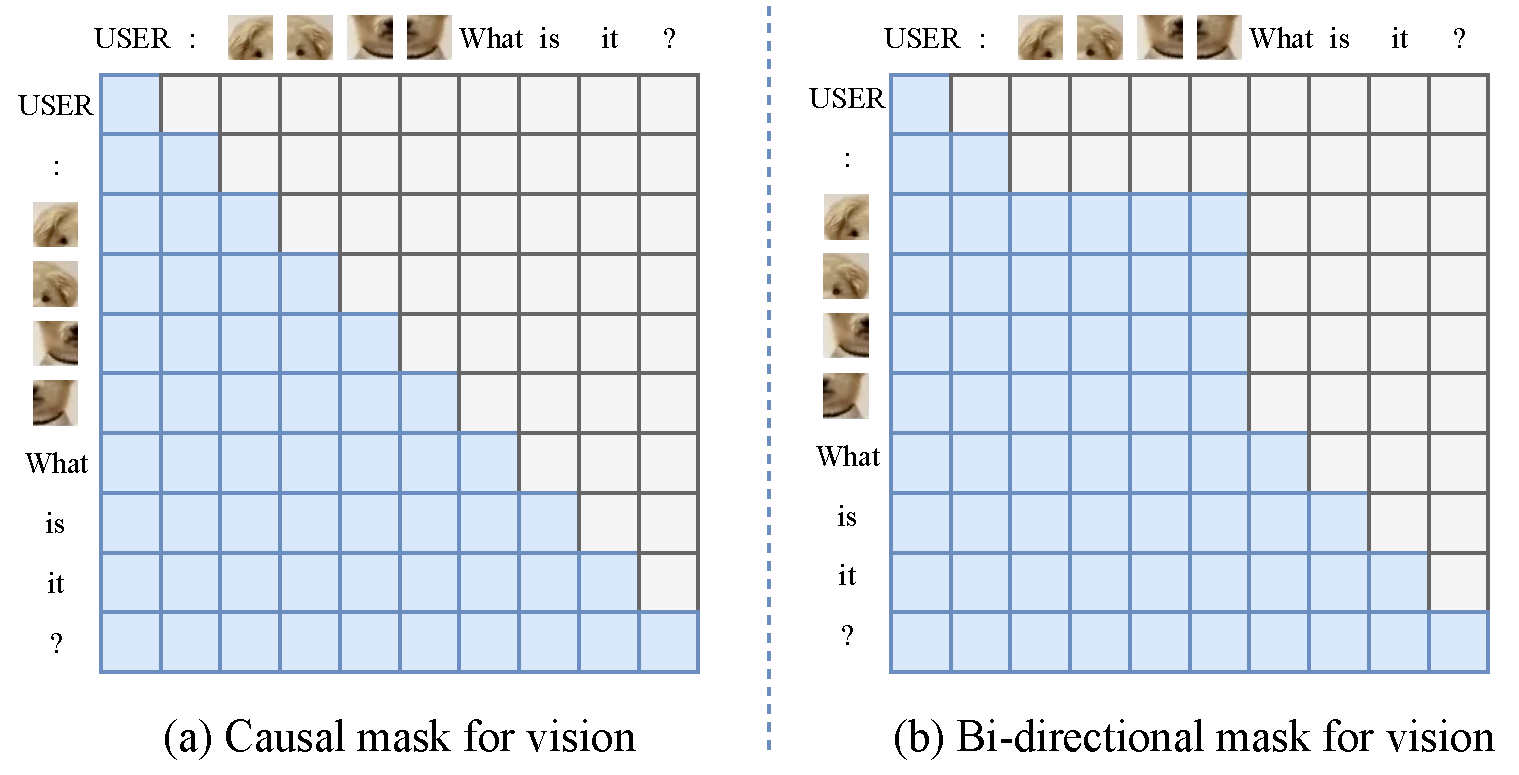
\includegraphics[width=\linewidth]{images/Figure3.pdf}
    \caption{Attention masks for vision: (a) causal attention inherits the autoregressive mask from language modeling, enforcing sequential dependency between image patches; (b) bidirectional attention offers full visibility between all image patches within the same input, enabling global contextual awareness.}
    \label{fig:attention-mask}
\end{figure}

While bi-directional attention masks is common in Transformer architectures in various fields \cite{vit, clip, transfusion}, few studies have explored replacing the causal mask of autoregressive LLMs with a bi-directional mask, especially in the field of MLLMs.

As illustrated in Figure \ref{fig:attention-mask}, we have explored the use of a bi-directional attention mask for vision. Our findings indicate that this attention mask positively impacts the final performance of \model{}, which will be discussed in Section \ref{sec:experiments}. In contrast to prior works \cite{eve, evev2, monointernvl, fuyu}, which have relied on causal masking designed for autoregressive text generation, we demonstrate that adopting bi-directional attention for vision tokens while retaining causal masking for text, not only preserves language capabilities but also enhances visual performance. This aligns with insights from image generation research \cite{transfusion}, highlighting \model{}’s potential as a unified architecture for multimodal generation and understanding tasks.
% \\
% As shown in Figure \ref{fig:attention-mask}, we explored three types of attention masks for vision: (a) causal mask, (b) bidirectional mask, and (c) localized bidirectional mask. While the bidirectional mask demonstrates improved performance, we find that the localized bidirectional mask outperforms it by allowing tokens to focus exclusively on a single image without interference from other text.
% \subsection{Simple Image Patchifier}

% Since we employ \model{} to encode visual information, we can utilize a very lightweight image patchifier. For simplicity, we use the original image patchifier from ViT, along with a single linear layer to align the dimensions, resulting in less than 10M parameters.


